\chapter{Lab 4: Memory Management}

\section{Introduction}

Congratulations on reaching the final lab of the MOS project! You have
made a lot of progress in the past few weeks.

In this lab, we will see, how memory is managed in the MOS kernel, which includes:

\begin{itemize}
    \item How virtual memory (i.e. paging) works.
    \item Page Faults.
    \item Copy-on-write (CoW) pages.
\end{itemize}

Let's begin the journey!

\begin{note}
    \item This lab requires you to have the \texttt{vmm} and \texttt{cow} debugging options
    enabled. You can use the following command to enable them:
    \begin{minted}{bash}
cmake . -DENABLE_DEBUG_vmm=ON -DENABLE_DEBUG_cow=ON
    \end{minted}
    \item (Otherwise, you won't see important debugging messages)
\end{note}

\section{Related Source Files}

\texttt{MM} stands for \textit{memory management}, and is the subsystem
responsible for managing both virtual and physical memory in the kernel.

The \texttt{MM} subsystem is implemented by multiple files inside the \texttt{kernel/mm/}
folder. The source files we care about (in this lab) are:

\begin{itemize}
    \item \texttt{paging/}: contains the higher-level paging code, includes functions
          for allocating and freeing pages, and for mapping and unmapping virtual
          memory.
    \item \texttt{cow.c}: contains the implementation of copy-on-write pages.
    \item \texttt{mmap.c}: contains the implementation of the \texttt{mmap} system call.
\end{itemize}

\section{Paging and Page Tables}

As you have learned in the lectures, paging is a mechanism that allows the
operating system to map virtual memory addresses to physical memory addresses,
you should have also learned about a general overview of how the page table
structure looks like.

A typical page table entry (PTE) contains at least the following fields:

\begin{itemize}
    \item A \textbf{physical address}: This is the physical address of the page
          in memory.

    \item Several \textbf{permission} bits: These bits determine if the page
          can be accessed by the user-space programs, if it can be written to,
          and if it can be executed, they are usually called the \textbf{user},
          \textbf{W} and \textbf{X} bits.

          \begin{exercise*}{Think about it}
              \item What will these bits be set to, for a page that contains
              the kernel code?
              \item \dots How about the kernel's read-only data?
              \item \dots How about user-space code?
          \end{exercise*}

    \item A \textbf{present} bit: if this bit is set, it means that the page
          is currently in memory, and the page table entry contains the physical
          address of the page.

          If this bit is set, it usually means that the page is readable, with
          the help of the \textbf{user} bit mentioned above, we can determine
          if the page is readable by the user-space programs or kernel only.

          \begin{exercise*}{Think about it}
              \item What does it mean by `the page is currently in memory'?
          \end{exercise*}
\end{itemize}

\subsection{The Kernel Page Table}

After some theory, let's see what a page table really looks like in MOS, make
101\% sure that you have the \texttt{vmm} debugging option enabled, and then start
the kernel in QEMU:

\begin{minted}{bash}
    qemu-system-i386 \
        -kernel mos_multiboot.bin \
        -initrd initrd.cpio \
        -m 4G -serial stdio
\end{minted}

\begin{exercise}
    \item Just before the output `\textbf{Welcome to MOS!}' and after
    `\textbf{Kernel Page Table:}', you should see a bunch of addresses and
    something looks like \texttt{rw-} or \texttt{r--}, this is a dump of the
    page table of the kernel.

    \item Given the fact that the kernel code starts at the virtual address
    \texttt{0xC0000000}, and the kernel heap starts at \texttt{0xD0000000},
    can you determine which column in the dump corresponds to the virtual
    address, and which one is the physical address?

    \item{} [Extension] There are two types of kernel data: read-only data,
    and read-write. Can you spot the difference between them in the page table dump?
\end{exercise}

\begin{figure}[htbp]
    \centering
    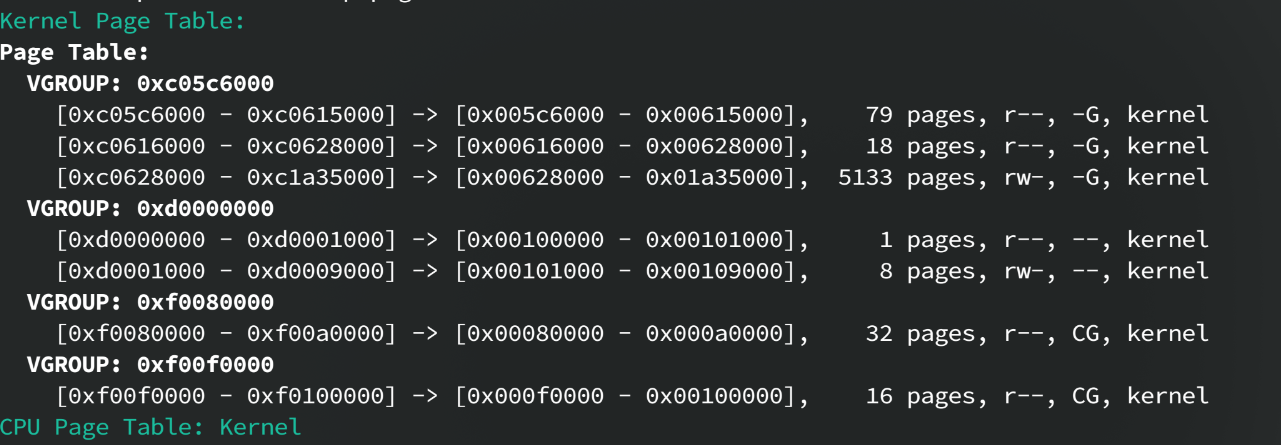
\includegraphics[width=0.8\textwidth]{assets/c4.page-table-dump.png}
    \caption{A dump of the page table of the kernel.}
    \label{fig:mm_dump_pagetable}
\end{figure}

\subsection{The User Page Table}

In the previous exercise, you should have noticed the last column only contains
`kernel'. This is because the dump happens before we even create the first user
process, and even before the kernel is fully initialized.

A normal kernel doesn't always dump the page table for you, so let's write a
system call that allows us to do that.

\subsubsection{System call definition table (\texttt{ksyscall.json})}

The first step is to add a new system call. Open the file \texttt{ksyscall.json},
one system call definition looks like this:

\begin{minted}{json}
    {
        "number": 42,
        "name": "my_syscall_name",
        "return": "bool",
        "arguments": [ { "type": "my_type_t", "arg": "my_arg" } ]
    },
\end{minted}

\begin{exercise}
    \item Write the syscall definition of \texttt{dump\_pagetable}, that takes
    \textbf{no} arguments, and returns \textbf{nothing}. (note that the syscall
    number should be unique)
\end{exercise}

\subsubsection{System call handlers (\texttt{ksyscall.c})}

This table contains the actual implementation of all system calls in MOS. One
system call handler looks like this:

\begin{minted}{c}
bool define_syscall(my_syscall_name)(my_type_t my_arg)
{
    // implementation...
}
\end{minted}

\begin{note}
    \item At first glance, this function may look a bit strange.

    \item But don't worry, the \texttt{define\_syscall()} macro is just a
    C macro that prepends a `\texttt{impl\_syscall\_}' to the function name.

    The full function declaration looks like this:

    \begin{minted}{c}
bool impl_syscall_my_syscall_name(my_type_t my_arg);
    \end{minted}

    \item This is to prevent name conflicts, since system calls may have the same
    name as other functions in the kernel.
\end{note}

\begin{exercise}
    \item Implement the system call handler for \texttt{dump\_pagetable}.
\end{exercise}

There are several helpers that you can use to implement this system call:

\begin{itemize}
    \item \texttt{current\_process}: the PCB of the current process, which contains
          a field called \texttt{pagetable}.
    \item \texttt{mm\_dump\_pagetable}: the function for dumping a page table.
    \item \texttt{mm\_dump\_current\_pagetable}: the function for dumping the page
          table of the current CPU, which usually is the page table of the current
          process.
\end{itemize}

\subsubsection{Recompile and test your implementation}

The next important step is to recompile the kernel so that the new system call
is available to user-space programs, and finally test it.

\begin{exercise}
    \item Recompile the kernel, (and fix any compilation errors).
    \item Start QEMU with \texttt{-append 'init=/initrd/tests/lab4.1'}.
    This will run our test program \texttt{lab4.1} as the init process.
\end{exercise}

If everything goes well, you should see the page table dump of the test program.
(see Figure \ref{fig:user_mm_dump_pagetable} for an example)

Otherwise, if you see a kernel panic complaining \texttt{init process exited with code 1},
and there is a message `\texttt{SYSCALL\_dump\_pagetable is not defined}', it means
either you didn't have the syscall named correctly, or you didn't recompile the kernel.

\begin{figure}[htbp]
    \centering
    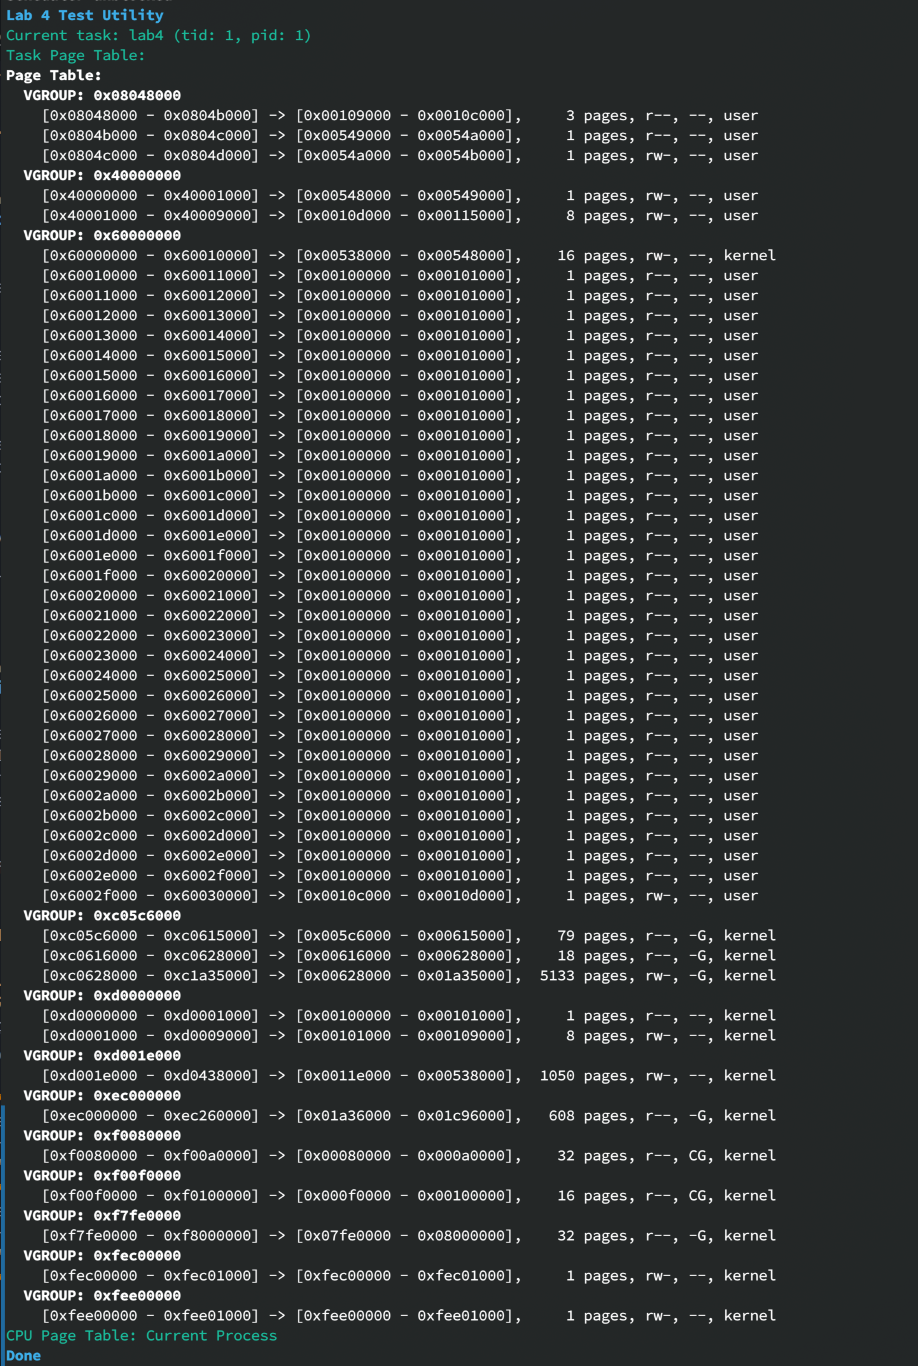
\includegraphics[width=0.9\textwidth]{assets/c4.user-page-table-dump.png}
    \caption{A dump of the page table of the user process.}
    \label{fig:user_mm_dump_pagetable}
\end{figure}

\begin{exercise*}{Think about it:}
    \item Where is the code, data, stack and heap of the \texttt{lab4.1} process
    located in the virtual address space?
    \item What is the difference between this page table and the one you saw
    in the previous exercise? What additional information does this page table
    contain?
    \item Why are there so many virtual pages mapped to the same physical page, and
    they are all marked as read-only?
\end{exercise*}

\subsection{Page Table Switching}

Different processes have different page tables, where the virtual addresses are
mapped to different physical addresses. The kernel will switch the page table
when the thread being switched to belongs to another process so that the addresses
are \textbf{isolated} from each other.

However, the kernel itself also needs paging to work, so it must have a page table
as well.

\begin{exercise*}{Think about it:}
    \item Where is the kernel page table located?
    \item If the kernel page table is \textit{stored separately} from the user page table:

    When does the `\textbf{switch}' happen, and where should the code, that
    does the switching, be located? Can it be in the kernel, or should it be
    in the user-space?

    \item If the kernel page table is \textit{\textbf{part} of} the user page table:

    How can the kernel page table be protected from being modified by the user
    process?
\end{exercise*}

The answer is, the kernel page table is \textbf{part of} the user page table, and
is always exactly the same across all processes. The only thing that makes kernel
addresses \textbf{kernel}-ish, is the permission bit \textbf{user} being unset.
This ensures normal user-space processes cannot access kernel memory.

Given the fact that the kernel pages are protected by the permission bit, there must
be a point where the CPU changes its working state to \textbf{kernel mode} so that
kernel pages become accessible. But when does this happen?

\begin{note*}{The CPU Black Magic}
    \item The answer is, it happens after a system call interrupt is triggered,
    but before the system call handler is executed, the transition happens
    entirely inside the CPU and is \textbf{invisible} to the outside world.

    \item There is a special structure which specifies that the CPU should
    switch to `\textbf{kernel mode}' before executing the interrupt handler.
    Then, when the handler returns, the CPU will switch back to its previous
    working mode, in our case, the `\textbf{user mode}'.

    \item We usually call this operation \textbf{`trapping' into the kernel}.
\end{note*}

\section{Page Fault}

A `page fault' is an interrupt that is triggered when the CPU tries to access a
page that is either:

\begin{itemize}
    \item Not mapped to any physical address, i.e. \textbf{present} bit is unset.
    \item Writing to a read-only page, i.e. \textbf{W} bit is unset.
    \item Accessing a page that is kernel-only, i.e. \textbf{user} bit is unset.
    \item Executing the code in a non-executable page, i.e. \textbf{X} bit is unset.
\end{itemize}

In such cases, the CPU saves the address that caused the fault, and turns back
to execute the page fault handler in the kernel for help.

It is then the kernel's responsibility to decide what to do with the faulting
address, and choose to either:

\begin{itemize}
    \item Map the address to a physical page and continue the execution.
    \item Kill the process and report the error to the user.
\end{itemize}

\section{Copy-on-write}

Copy-on-write (or CoW for short) is a technique that allows the kernel to
\textbf{delay} the copying of a page's content until it is actually modified.

\subsection{Why do we need CoW?}

When a process asks the kernel either to \texttt{fork}, or to allocate
a new block of memory, it is unlikely that the process will immediately
modify all the memory it just allocated.

Therefore, it is a waste of physical memory to copy the content
immediately, or zero out the newly allocated memory.

The copy-on-write technique allows the kernel to delay the copying,
until the child process actually modifies the pages.


\subsection{How does CoW work with paging?}

The CoW is relatively easy to implement with paging, only a few steps are needed:

\begin{enumerate}
    \item When a process asks the kernel to allocate a new page or to fork, the kernel,
          depending on the situation, may choose to:
          \begin{itemize}
              \item Map the virtual address to a \textbf{zero page}, which is a
                    page that contains only zeros, this is the case when the
                    process asks for a new page of memory.
              \item Map the virtual address to a \textbf{physical page}, which is
                    a page that is already mapped to another process, this is the
                    case when the process asks to \texttt{fork}.
          \end{itemize}
    \item The kernel marks the page as \textbf{read-only}, so that
          writes to the page will trigger a page fault.

          In the case of \texttt{fork}, the kernel also marks the page in
          the parent process as \textbf{read-only}, so that either process
          can trigger a page fault.

    \item When a page fault is triggered by writing to the page, the
          kernel allocates a new physical page, copies the content from the
          zero page, and \textbf{re}maps the virtual address to the new physical page.
    \item The kernel marks the new page as \textbf{read-write}, so that
          future writes to the page will not trigger a page fault.
    \item The kernel returns to the user process, the CPU will retry
          the instruction that caused the page fault, and this time it will
          succeed.
\end{enumerate}

In MOS, the zero page is allocated by the \texttt{mm\_cow\_init} function in
\texttt{kernel/mm/cow.c}. This function is called once during the kernel
initialization.

\begin{note}
    \item Some may call the zeroed page technique \textbf{Zero-fill-on-demand},
    which is a special case of CoW. But in MOS, we will just call it CoW.
\end{note}


\subsection{Resolving a CoW Page Fault}

In this section, we will walk through the steps of resolving a CoW page fault.
We will look at the function \texttt{do\_resolve\_cow}.

\begin{note}
    \item The \texttt{do\_resolve\_cow} function is called by the page fault
    handler, which is defined later in the same file.
\end{note}

The function gives a simple overview of how CoW can be resolved:

\begin{enumerate}
    \item Several sanity checks are performed before calling this function,
          such as checking if the page fault is caused by a write, and if the
          block of fault is actually a CoW page.
    \item The kernel allocates a new page and maps it to a temporary virtual
          address.
    \item The kernel copies the content from the old, faulting page to the new
          page it just allocated.
    \item The kernel \textbf{replace}s the old page with the new page, by
          modifying the page table entry, with the new physical address and
          its original permission bits.
    \item The kernel \textbf{unmap}s the temporary virtual address.
\end{enumerate}

\begin{exercise*}{Implementing \texttt{do\_resolve\_cow}}
    \item Although the function is already implemented, try removing
    the code in it and see what happens.
    \item Can you re-implement the function by yourself?

    Run QEMU with \texttt{-append 'init=/initrd/tests/lab4.2'} to test your
    implementation.
\end{exercise*}

\subsection{Allocating a Zeroed Page}

Allocation of a zero page is relatively simple, the kernel just needs to
find a new virtual address and map it to the zero page. This is done by
\texttt{mm\_alloc\_zeroed\_pages}.

The current implementation of \texttt{mmap} does not allocate a zero page
for the process, instead, it allocates a physical page and returns to
the user without zeroing it.

This is inefficient because if the user requests a large number of pages but
only uses one or two of them, the kernel will waste a lot of physical memory
to store unused pages.

Even worse, the non-zeroed pages may contain sensitive information from
other processes, which is a security risk.

\begin{exercise}
    \item Modify the \texttt{mmap\_anonymous} function in \texttt{kernel/mm/mmap.c},
    so that it uses CoW to allocate a zero page for the process.
    \item Run QEMU with \texttt{-append 'init=/initrd/tests/lab4.3'} to test your
    implementation.

    Your implementation should pass the test, as shown in Figure \ref{fig:lab4.3}.

    \begin{figure}[H]
        \centering
        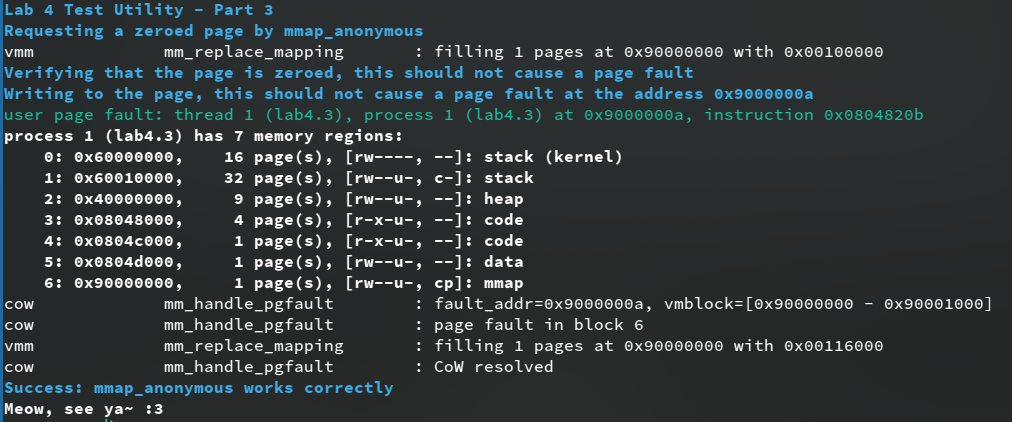
\includegraphics[width=0.8\linewidth]{assets/c4.mmap.png}
        \caption{Lab 4.3 Test Result}
        \label{fig:lab4.3}
    \end{figure}
\end{exercise}

\section{Extension: Copy-on-Write Things}

There are several questions you can think about, as an extension to this lab and to
strengthen your understanding of CoW:

\begin{itemize}
    \item In the current implementation, the kernel stack is allocated without
          using CoW, why is that?

          \textbf{Hint}: Think about when an interrupt occurs, and the kernel
          needs to use the kernel stack to handle the interrupt. What if the
          kernel stack is a CoW page?

    \item It seems that CoW is a very useful technique, but is there a case
          where CoW is not useful?

          \textbf{Hint}: Interrupt takes time, and CoW is no exception.
          There are cases where a process immediately modifies one page after it is
          allocated, can you find such a case?

          Is there a way to avoid CoW in this case?

    \item Can we use copy-on-write on the page table itself?

          (I don't know the answer)
\end{itemize}
